\documentclass[10pt]{article}

% to compile a camera-ready version, add the [final] option, e.g.:
\usepackage[final]{report_template}

% to avoid loading the natbib package, add option nonatbib:
% \usepackage[nonatbib]{neurips_2020}
\usepackage{mathptmx}
\usepackage[utf8]{inputenc} % allow utf-8 input
\usepackage[T1]{fontenc}    % use 8-bit T1 fonts
\usepackage{hyperref}       % hyperlinks
\usepackage{url}            % simple URL typesetting
\usepackage{booktabs}       % professional-quality tables
\usepackage{amsfonts}       % blackboard math symbols
\usepackage{nicefrac}       % compact symbols for 1/2, etc.
\usepackage{microtype}      % microtypography
\usepackage{graphicx}
\usepackage{xcolor}
\usepackage{wrapfig}
\usepackage{subcaption}

\title{Detection of Mineral Deposits in NASA \emph{LandSat}
        Images Using Convolutional Neural Networks}

\author{
  Sean McAuliffe, V00913346
  \And
  Spencer Davis, V00759537 
  \And
  Kiana Pazdernik, V00896924 
  \And
  Mateo Moody, V00918050 
  \And
  Chris Wong, V00780634 
}

\graphicspath{{./figures/}}

% \begin{figure}
%   \centering
%   \includegraphics[width=0.65\linewidth]{1.jpg}
%   \caption{Sample figure caption.}
%   \label{fig:1}
% \end{figure}

\begin{document}

\maketitle

\begin{abstract}
  We trained Convolutional Neural Networks (CNNs) to identify locations likely
  to contain useful mineral deposits on the Earth's surface using NASA Landsat
  Earth observation images. Training labels for supervised learning were generated
  programmatically using a corresponding dataset of known mineral deposits. AI
  assistance in locating mineral-rich locations can potentially help to minimize
  the environmental impact caused by prospecting and mineral extraction, which
  is generally harmful to the environment and human health. The Landsat
  dataset is preprocessed by downsampling to a resolution of 512x512. The images
  are labelled using a K-D Tree Search Algorithm into the minerals dataset. Both
  binary classification and regression labels were generated for all images.
  Sets of labelled images are organized into buckets based on their location.
  Ocean masking is performed to remove buckets over open water to prevent the
  resulting ML agent from simply learning to distinguish between land and sea.
  The images at each location are then sorted by degree of cloud cover, allowing
  for the selection of training images with minimal cloud cover. Once the images
  are preprocessed, they are split into training and testing sets for supervised
  learning. Several combinations of model architectures and hyperparameters
  were investigated to find a model which achieved high accuracy. For evaluation
  purposes, all models were compared against a baseline obtained by training the
  model on a training set with randomized labels. The trained models obtained an
  accuracy of 73\% on the binary classification problem, and a MAE of 0.117 on
  the regression problem; these values both represent notable improvements over
  baseline. Training on more powerful hardware and using the full-resolution
  images may produce further improvements.
\end{abstract}

\section{Introduction}

\subsection{Problem Description}

The work of prospecting for mineral deposits is complicated and can be dangerous.
In some cases it can be harmful to the environment and human health. Current
techniques depend on specific geological knowledge, and utilize a combination of
magnetic, gravimetric radiometirc, and seismic methods. Our work proceeds from
curiosity; can AI assistance be used to learn generalizable patterns — as of yet
unknown to human geologists — that emerge in surface features, which may be highly
predictive in identifying useful mineral deposits?

\subsection{Approach}

This project was conceived, in part, to take advantage of the extensive Landsat
dataset, which is freely available and contains over 8 million Earth observation
scenes taken over the past 50 years [1]. Landsat images are very high resolution,
as such, Convolutional Neural Networks were chosen as the primary learning agent
for this project. 

Convolutional Neural Networks have proven to be very effective in image classification
tasks [2]. Of particular interest to this project is the ability of CNNs to
quickly reduce the resolution of an image, while preserving learned patterns.
This is useful for our project, as the Landsat images are very high resolution,
and would be difficult to train on using a consumer GPU.

The Landsat dataset was combined with a dataset of known mineral deposits to
generate training labels for supervised learning; the label of each image
indicated the presence or richness of minerals in the image.

Much of the work involved in this project was in the preprocessing and problem
setup. These steps anticipated and attempted to remove sources of error, and to
constrict the the problem such that the ML agent would learn to identify useful
patterns. For example, algorithms were devised to identify and select training
images having a minimal level of cloud cover, and to exclude images taken
over water. The full details of the preprocessing pipeline can be found
in section \ref{sec:pf}.

\subsection{Goals}

We aim to train Convolutional Neural Networks to achieve 80\% validation accuracy
on the binary classification problem, and a Mean Absolute Error of $\leq 0.1$
on the regression problem.

\section{Problem Forumulation}\label{sec:pf}

The problem formulation step encompases the bulk of the work. This step prepares
the data for the model to train on. The particular ways in which the dataset
is chosen, labelled, and prepared effect what the model will learn. These
decisions are made with the goal of constraining the problem in such a way that
the model will learn to solve the problem as formualted in our minds. Each
formulation rests on a particular philosophy of what should be learned, and each
has its own strengths and weaknesses.

We formulated the problem in two ways: binary classification, and regression. Each
is described in the following subsections. Both approaches shared much of the
same acquisition and preprosccesing pipeline as described below.

\subsection{Data Acquisition \& Preprocessing}

\begin{wrapfigure}{r}{0.4\textwidth}
  \centering
  \includegraphics[width=0.38\textwidth]{1.jpg}
  \caption{\textit{An example Landsat image in band 7.}}
  \label{fig:example_image}
\end{wrapfigure}

We acquired the entire set of approximately 45000 band 7 images from Landsat 4 of the
\href{https://console.cloud.google.com/marketplace/product/usgs-public-data/landast}{\textcolor{blue}{\underline{public Landsat dataset}}}
on Google Cloud Platform. We chose band 7 (2.09-2.35$\mu$m) because it uses a
Thematic Mapper sensor to capture light in frequencies optimal for identifying
hydrothermally-altered rocks associated with mineral deposits. These images are
each approximately 7500x7500 pixels in a single colour channel, and are taken
at regular locations on a 2x2$^\circ$ latitude-longitude grid.

We also acquired a \href{https://www.kaggle.com/datasets/thedevastator/mineral-ores-around-the-world}{\textcolor{blue}{\underline{dataset}}}
of approximately 350000 mineral deposits, each including the deposit's coordinates
and the types of minerals present. 

% For each of the following: describe what problem exists, and how it is resolved

% Download from the cloud 

We automated the image downloads using a bash script. This script used the
bash utility \emph{ImageMagick} to downsample each image from 7500x7500 to 
approximately 512x512, to allow for training on consumer hardware. The
corresponding metadata file for each downloaded image was also obtained,
containing information such as the coordinates of the image corners. The download
took approximately 6 seconds per image, for a total download time of approximately
75 hours.

% Downsampling techniques

Several differen algorithms from were experimented with: resizing,
rescaling, and sampling. Resizing and rescaling use similar  iterative processes of
averaging neighboring pixels to effectively compress the image while reducing quality.
Sampling is a more direct approach which simply selects a subset of the pixels
evenly from across the input image. This is the lossiest of the three methods,
but is also the fastest. The results of these three methods are shown in 
Figure \ref{fig:downsample}.

\begin{figure}
  \centering
  \begin{subfigure}{0.22\textwidth}
      \centering
      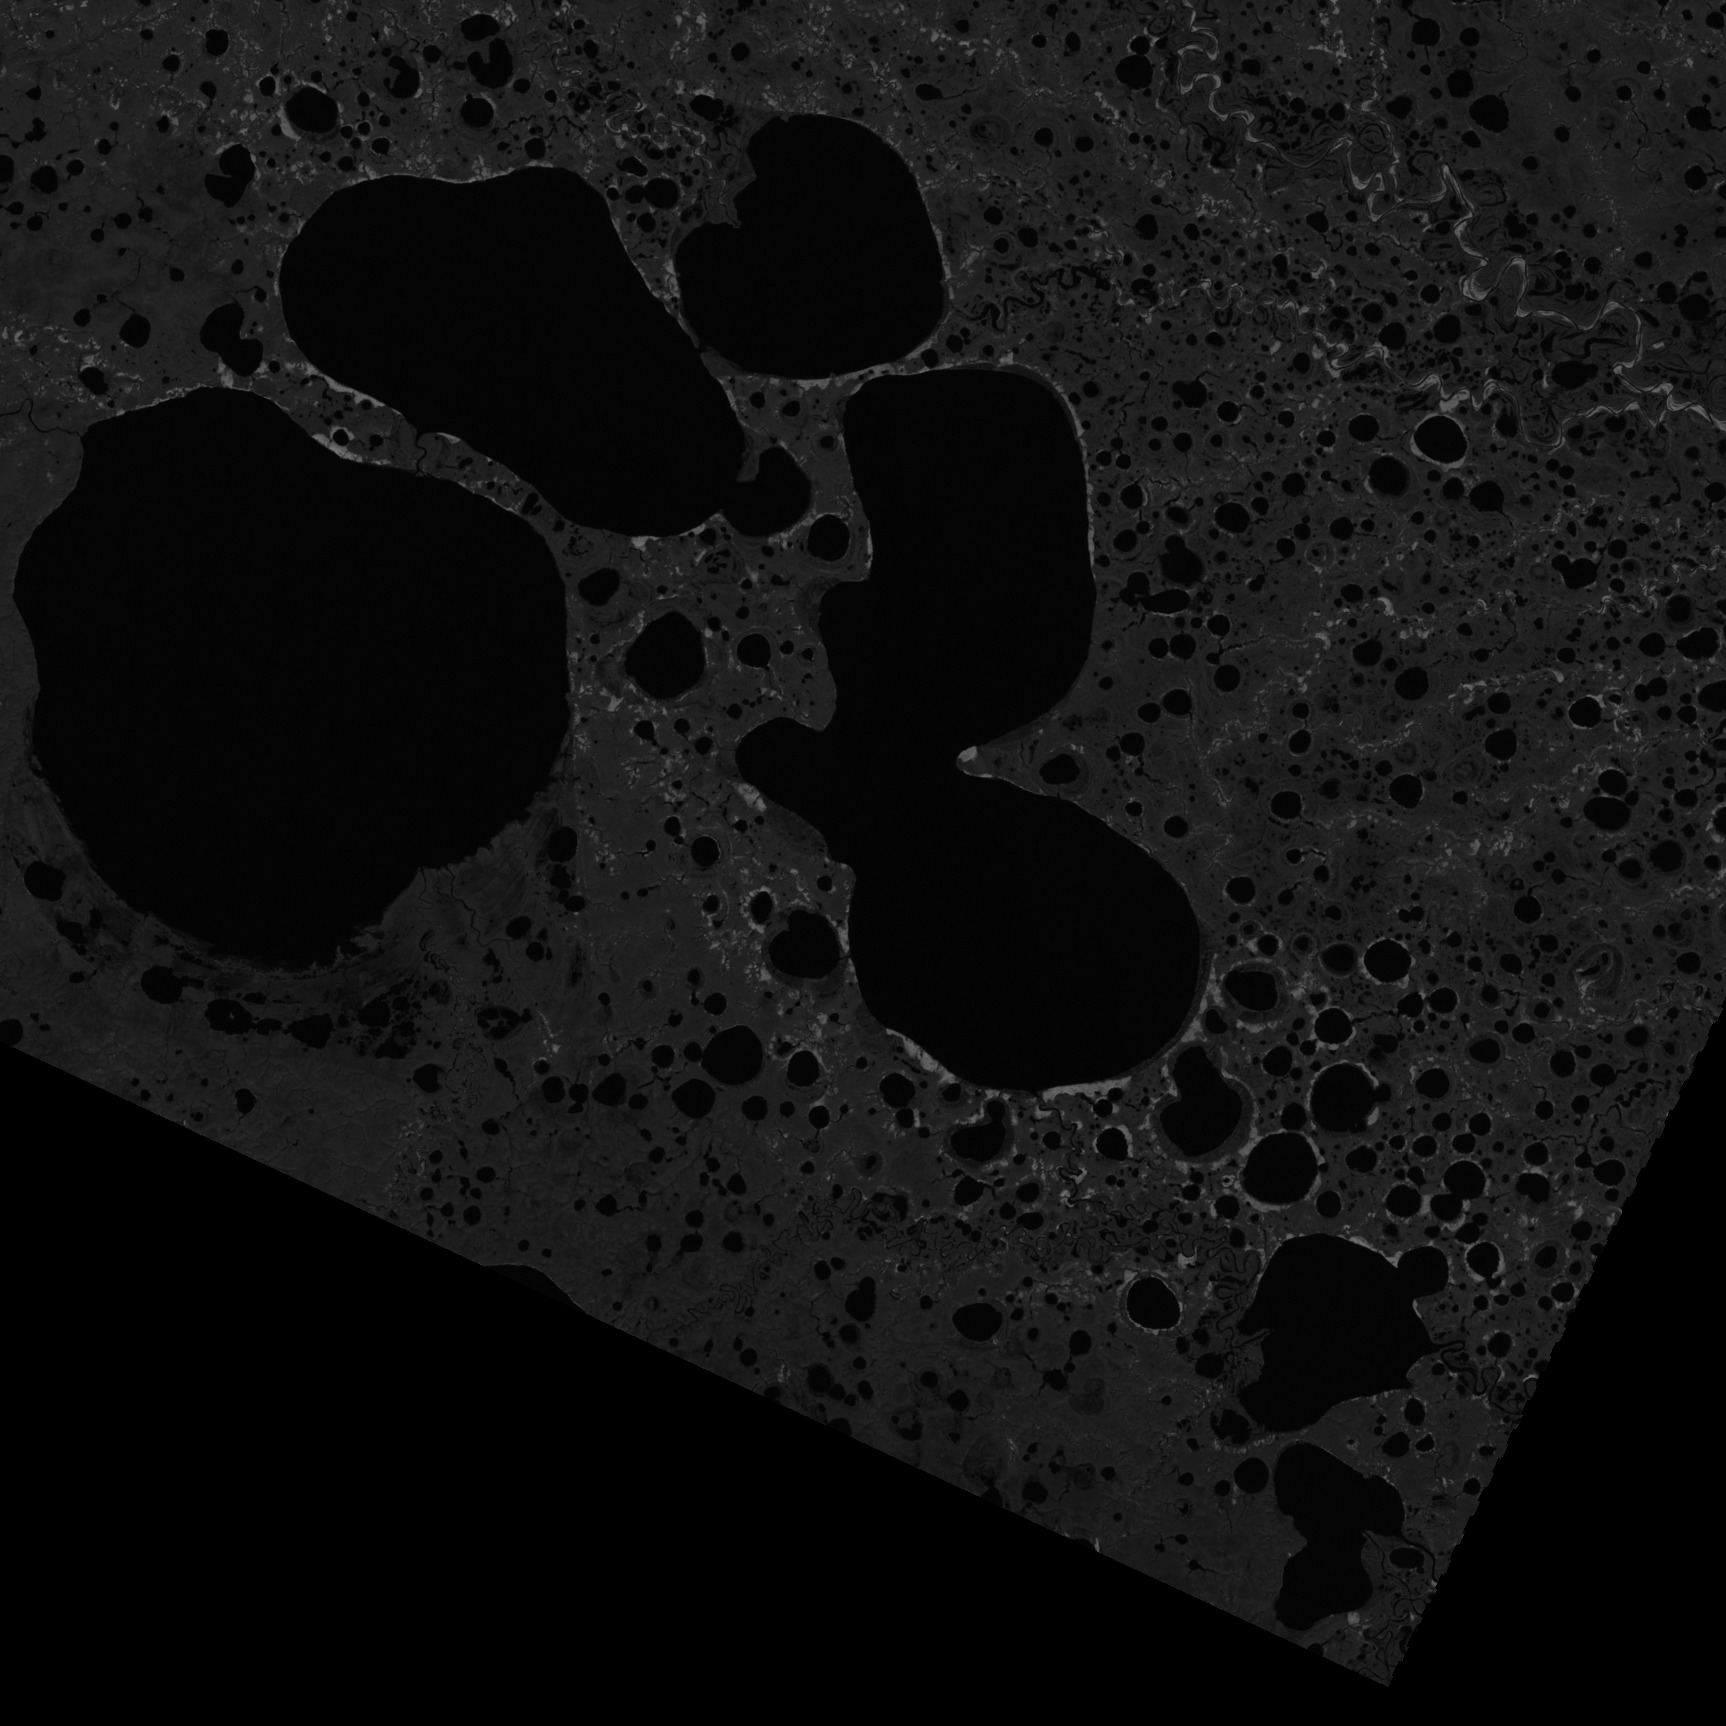
\includegraphics[width=\linewidth]{original_good.jpg}
      \caption{\textit{Original}}
      \label{fig:image_1}
  \end{subfigure}
  \hfill
  \begin{subfigure}{0.22\textwidth}
      \centering
      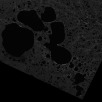
\includegraphics[width=\linewidth]{rescale_good.jpg}
      \caption{\textit{Rescaled}}
      \label{fig:image_2}
  \end{subfigure}
  \hfill
  \begin{subfigure}{0.22\textwidth}
      \centering
      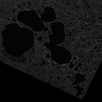
\includegraphics[width=\linewidth]{resize_good.jpg}
      \caption{\textit{Resized}}
      \label{fig:image_3}
  \end{subfigure}
  \hfill
  \begin{subfigure}{0.22\textwidth}
      \centering
      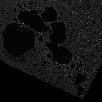
\includegraphics[width=\linewidth]{resample_good.jpg}
      \caption{\textit{Downsampled}}
      \label{fig:image_4}
  \end{subfigure}
  \caption{Three compression techniques applied to the same Landsat image}
  \label{fig:downsample}
\end{figure}

% Label Creation

Labels were created for each image using an algorithm accelerated by a
k-d tree of mineral deposit locations; the k-d tree was used since k-d trees
provide significant speedup for queries on spatial data [3]. Efficient label creation
was nontrivial since it required identifying which mineral deposits were present
in each image, and the images were neither axis-aligned nor perfectly rectangular.
To address this, the label-creation algorithm first computed the enclosing circle
of each image, then queried the k-d tree for the set of deposits present in the circle;
brute force was then used to test which of these deposits were within the convex
polygon of the image. This method provided a speedup of 20x over the naive approach.

\begin{figure}[ht]
  \centering
  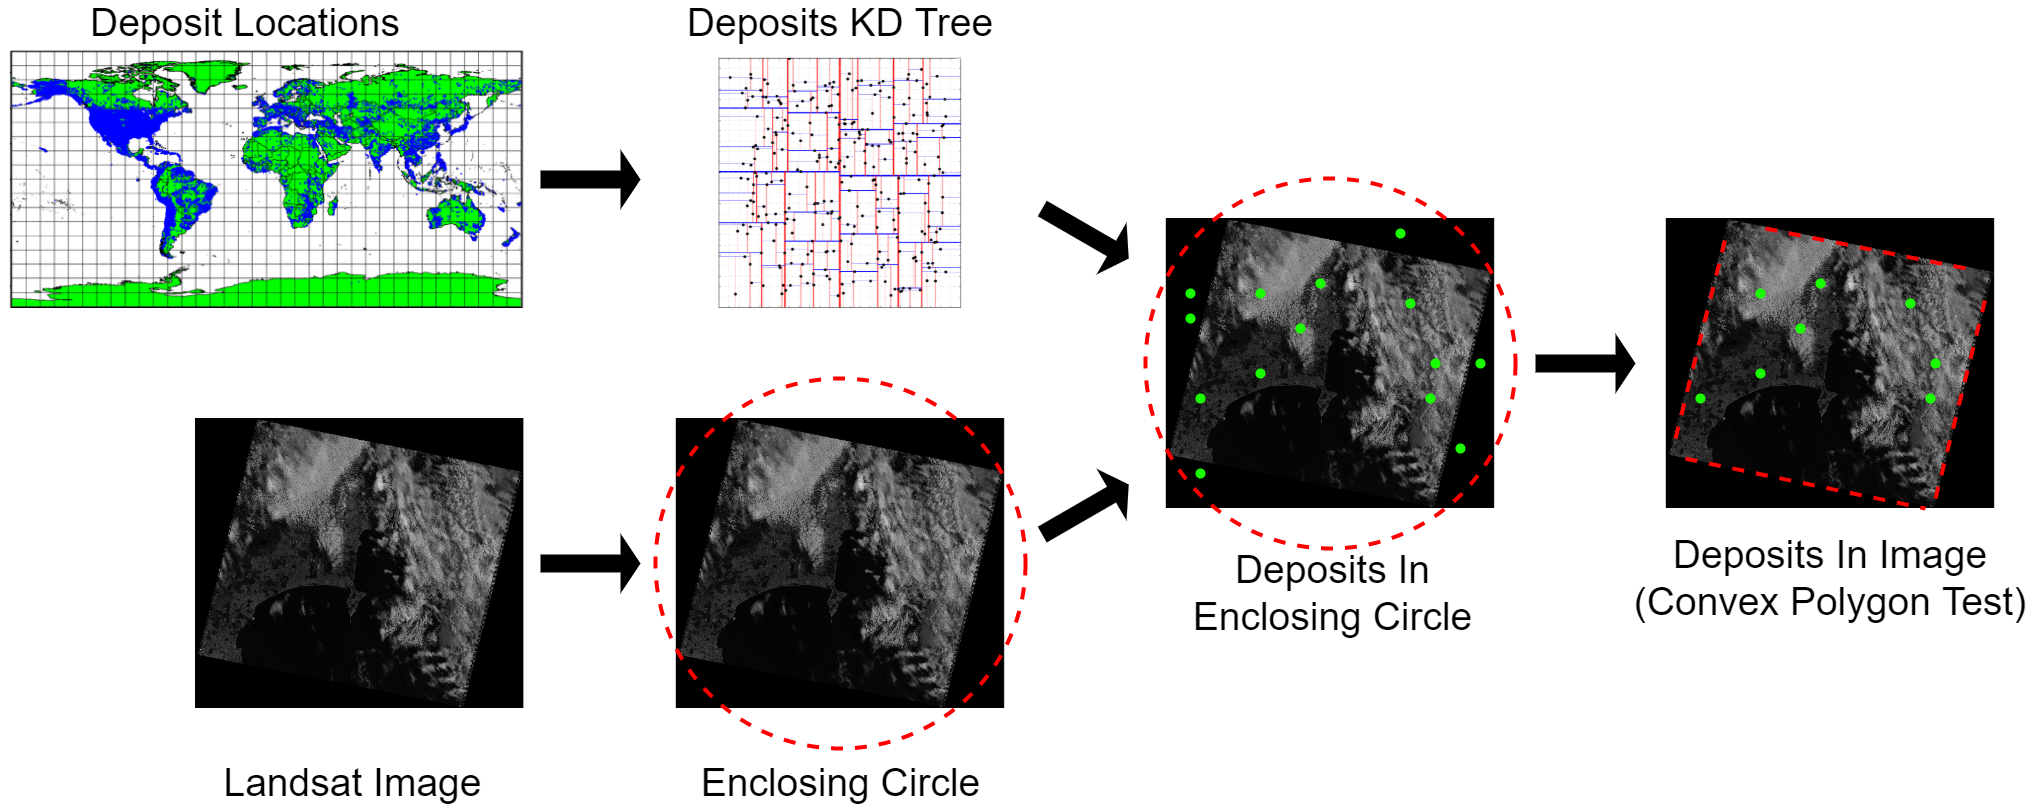
\includegraphics[width=\linewidth]{label-creation.png}
  \caption{Label creation pipeline}
  \label{fig:2}
\end{figure}

\begin{wrapfigure}{r}{0.45\textwidth}
  \centering
  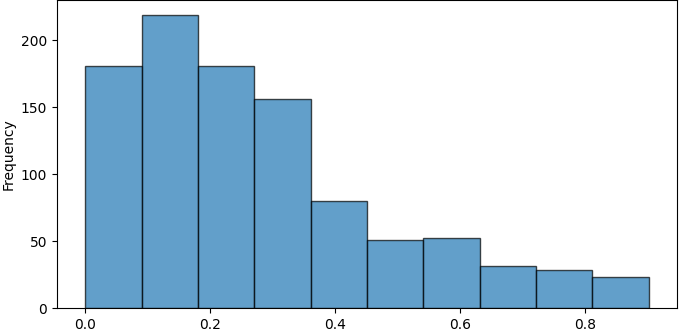
\includegraphics[width=0.38\textwidth]{good_histo.png}
  \caption{Distribution of log-normalised richness scores}
  \label{fig:histogram}
\end{wrapfigure}

Having obtained the set of deposits present in an image, separate labels were
created for binary classification and regression. The binary classification labels
indicated whether any minerals were present in the image, and the regression labels
indicated the mineral richness of the image. The richness score was computed as the
log transform of the absolute count of deposits in the image, normalized to the range 0-1.
The log transfrom was used to reduce the skew of the regression values.

\begin{equation}
label^{\prime}_i = \frac{\ln(label_i + 1)}{max(labels)}
\end{equation}

% Location buckets.

\paragraph{Location Buckets:} Since Landsat images are taken at regular intervals,
and our dataset contained several images at each location, it was necessary to
ensure that no location appeared in both the training and testing sets simultaneously.
To achieve this, the images were grouped by location, resulting in approximately
6000 unique location buckets.

% Cloud Cover

Having grouped the images by location, the images in each bucket were sorted
by average pixel brightness, which for band 7 images effectively sorts by degree
of cloud cover. This permits the selection of training images having less cloud cover.

% Ocean Masking

Finally, images in location buckets over the ocean were removed, to ensure that our models
did not learn to simply detect land. The Python library Geopandas was used to load
a \href{https://www.naturalearthdata.com/}{\textcolor{blue}{\underline{geospatial dataset}}}
containing the polygons of the boundaries of all land on Earth; this dataset was
then queried to determine whether each image's centerpoint was over land.

% Training and Testing Sets + proportions of labels

To prevent our models from simply learning the underlying distribution
of training labels, we ensured that the ratio of class labels in the training
set is balanced. In binary classficiation this is trivial, we enforce that
the training set be comprised of 50\% positive and 50\% negative labels. In
the regression case, the set of all examples has some underlying distribution
shown in figure \ref{fig:histogram}. The training set is then sampled randomly
(without replacement) from this distribution, and therefore comes to have a very
similar distribution. The remaining images are used as the validation set.

The training + testing set was drawn from the set of all images such that at least
one image from each location bucket was included. The training set was then
randomly sampled from this set, and the remaining images were used as the testing set.
All experiments used a 80/20 split between training and testing sets.

Finally, since the Landsat images vary slightly in size and are not perfectly square,
each image was padded to 512x512 pixels with black pixels, and all pixel brightnesses
were normalized to the range 0-1. 

\subsection{Binary Classification}

The binary classification problem setup was the first to be designed. It represents
the simplest formulation of the problem, and our naive initial understanding.
The primary goal of this problem was to determine whether a model trained
on the dataset described above could learn anything relevant to the problem which
would enable it to perform better than chance. To this end, examples with binary
labels were prepared for the model as described above. 

This approach initially proceded from the assumption that mineral deposits would
be sparesely located throughout the world, and that their presence might correspond
to certain easily detectable surface features. However, when the labelled location
buckets were later plotted on a world map it became obvious that there was
a clear preponderance of positive labels over land. Given the large surface area
covered by each image almost all images contain at least some small number of desposits. 

\begin{figure}[ht]
  \centering
  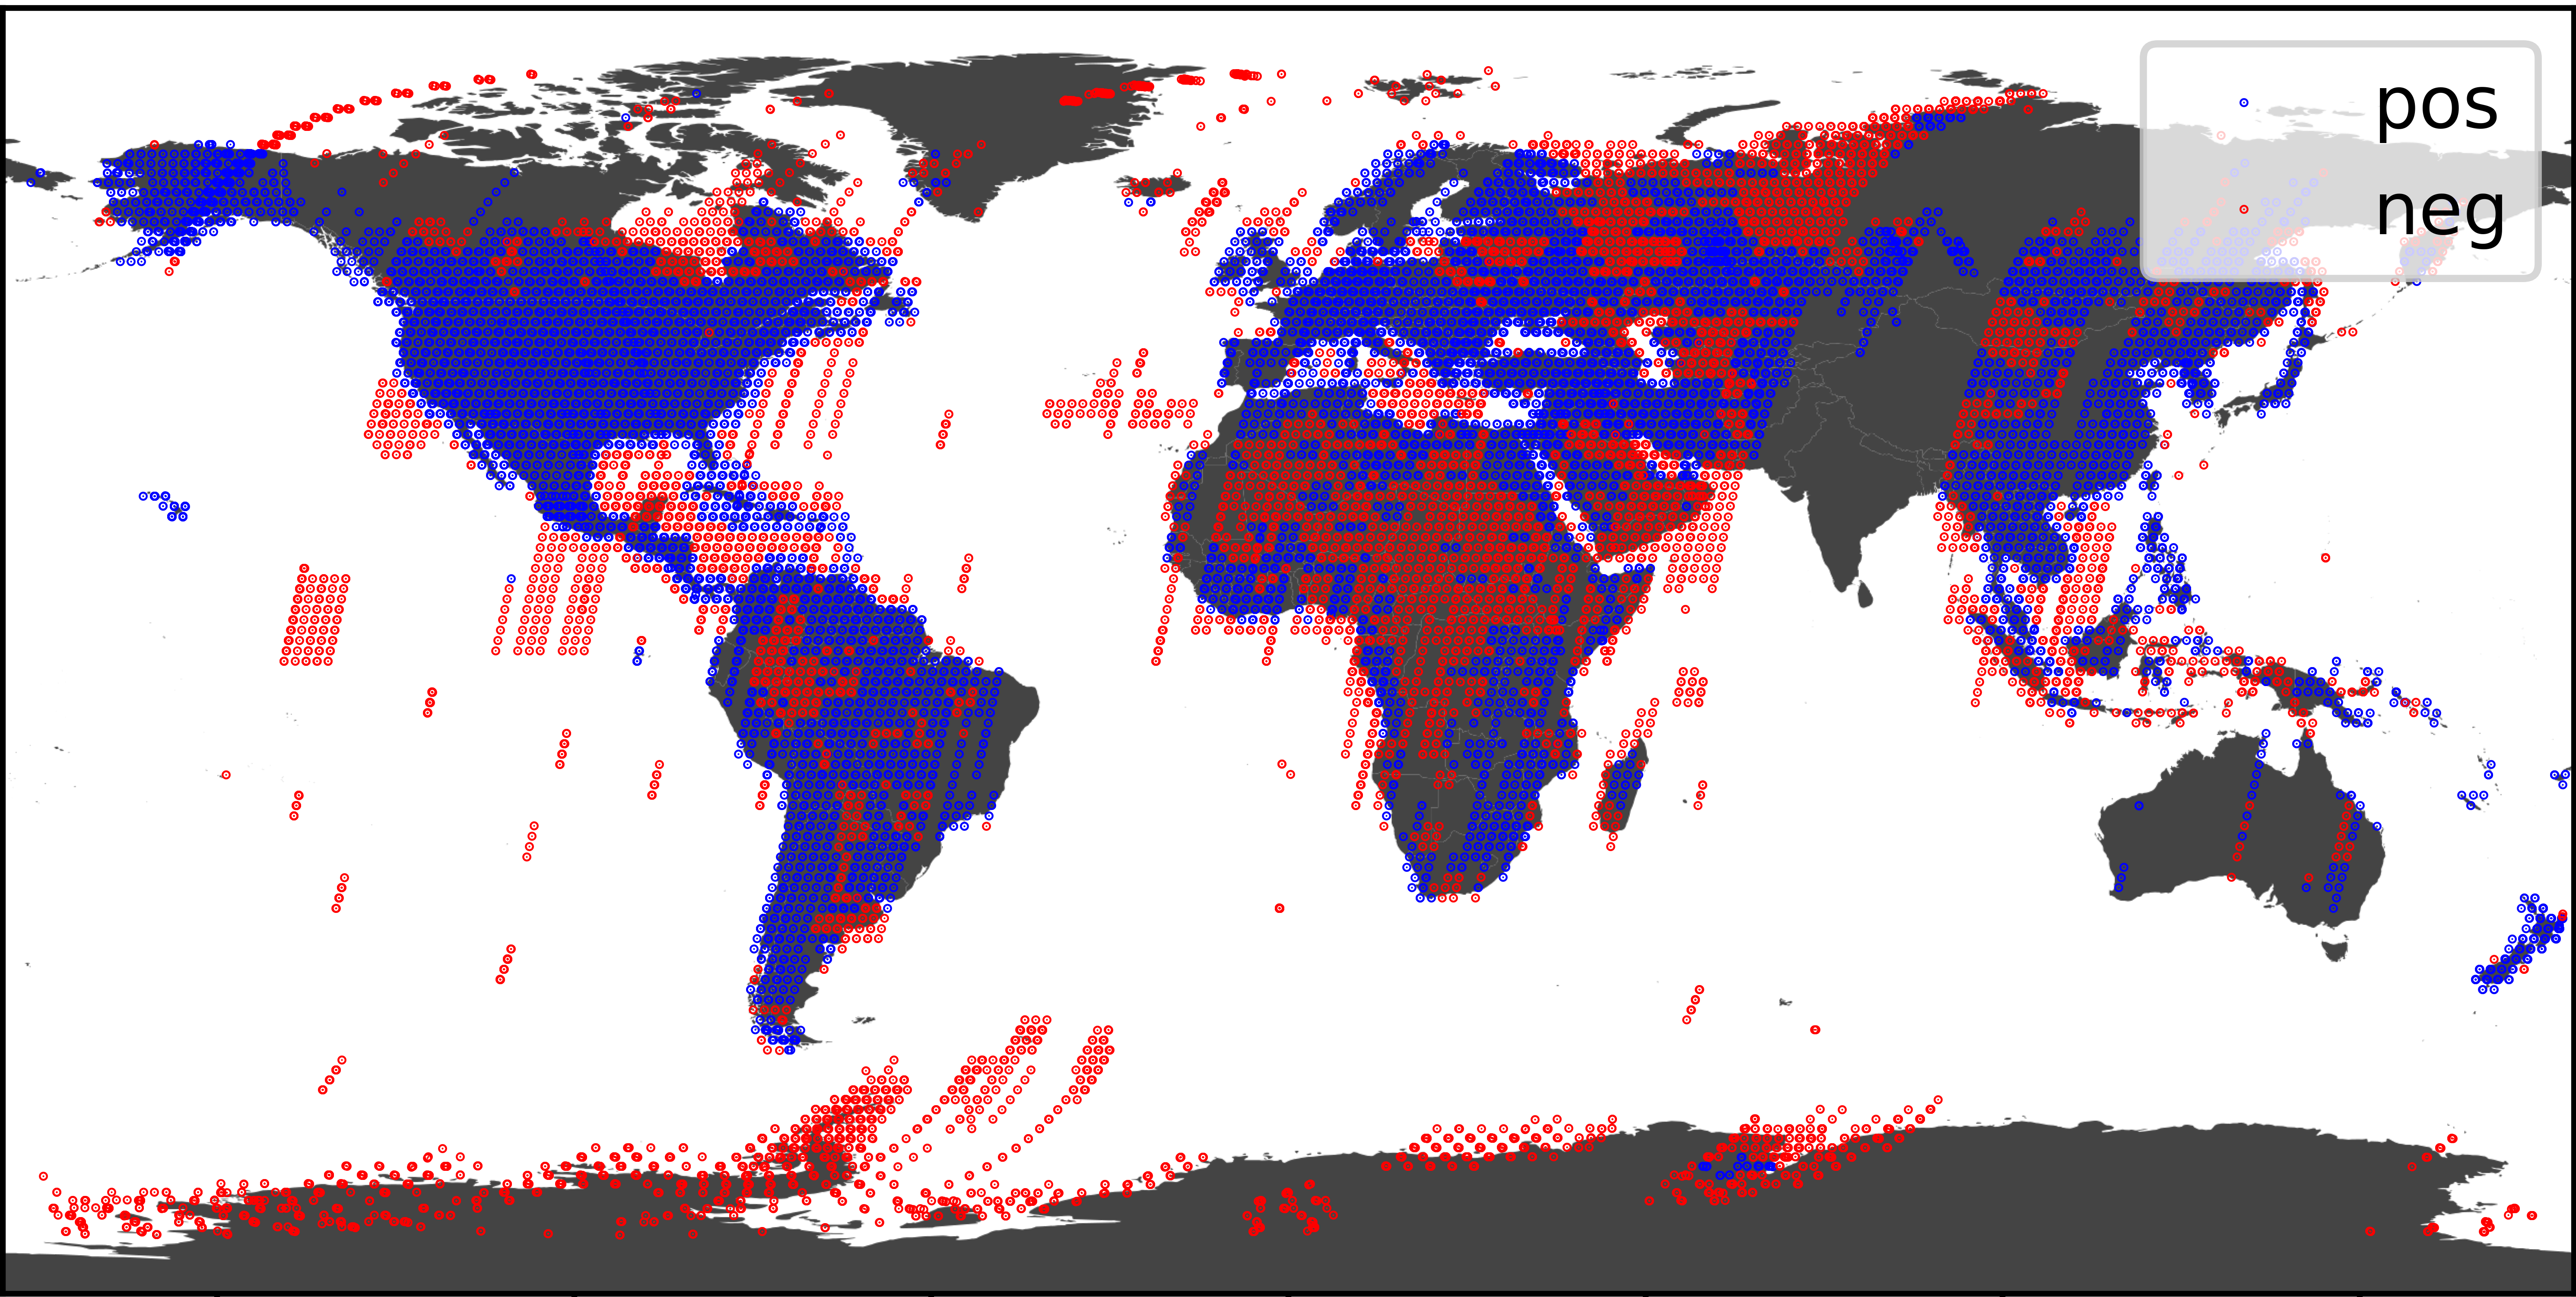
\includegraphics[width=0.75\linewidth]{locations.png}
  \caption{All labelled location buckets}
  \label{fig:locations}
\end{figure}

Additionally, negatively labelled images do not necessarily mean that there are
no mineral deposits in the region. In fact, this is a major philisophical problem
with the problem setup. Many of the false positives that the model will produce
may in fact be true positives representing new desposits which the model has
successfully identified. Without any way of independently verifying the 
presence of these deposits we are unable to truly evaluate the model's performance,
and the model could never further learn from these examples.

Nevertheless, this problem formulation does allow us to successfully determine
whether our dataset contains information which is learnable by a CNN. 

\subsection{Regression}

The regression problem was designed to address the issues with the
binary classification problem, and sought to investigate the feasibility of
the practical application of our methods. In practice, a predicted richness
score is more useful than a binary prediction when choosing a location to dig
for minerals. The regression formulation also addresses the problem of
whether negative examples are really negative: if a regression model
achieves a low error when trained only on examples containing known deposits,
then predicts a high richness score on an example containing no known deposits,
it may indicate the presence of undiscovered deposits.

To improve the interpretability of our regression model performance,
the training and testing sets for the regression problem were sampled
such that each had a near-equivalent distribution of label values.

\section{Background and Related Work}

Much of the previous work done to integrate satellite and aerial photography into
the mining industry has been to better assess geographic factors relevant as
obstacles to construction and extraction [4]. As well as to predict the extent of
damage down to the natural landscape, for instance, to determine if much tree cover would have
to be removed. Other work at automatically detecting minerals from orbit has been
limited by the sensor capabilities of the satellites, indeed typically only those
sensors with very high resolution and particular imaging wavelengths are useful
for geological applications. 

% https://www.satimagingcorp.com/applications/energy/mining/
% https://www.esri.com/about/newsroom/arcwatch/mineral-exploration-in-the-hyperspectral-zone/

% https://arxiv.org/pdf/2103.07678.pdf
% Other work has incorporated AI in the development of maps, and to search for
% particular features which geologists have decided apriori are correlated with 
% particular kinds of despits.

% Our work proceeds from the naively curious position of wondering if new patterns
% useful in predicting the location of deposits, as of yet unknown to geologists,
% could be learned by ML agents. Our work is limited by the resolution of the
% data and our computing power. A more exhaustive search of this question would
% train on multiple EM bands, and the full resolution available; and would likely
% achieve more impressive results. As it stands, we have learned some modest
% amount of information in the available dataset which does allow us to predict
% the extent of mineral richness depicted in an image ~8\%  better than chance.

\section{Methods}

% \begin{equation}
%   W(C) = \sum_{j=1}^{k} \sum_{x \in C_j} \lVert x - \mu_j \rVert^2
% \end{equation}

% quick blurb introducing the section
% Philosophy: explore architectures, then tune hyperparameters

\subsection{Model Architecture}

% Discuss in DETAIL the model architecture --> refer to keras documentations 
% generate some equations and diagrams which explain what each layer does 
% why it was included (what problem we hoped it would solve).

% Describing the theory behind the keras implementation of CNNs 

% Discuss our model architecture search space plan (small, medium, large)

\subsection{Hyperparameter Tuning}

% Describe the math behind each of the hyperparameters 

% Discuss the meaning of each of the hyperparmaters

\subsection{Model Evaluation}

% Discuss the metrics and loss functions used to train + evaluation the model
% show the MATH

% Discuss that each model was compared against a baseline of randomized labels
% to determine if the model was learning anything at all

\section{Results}

% Quick blurb 

\subsection{Binary Classification}

% Discuss the results of the architecture and hyperparameter searches 
% include graphs of model accuracy

\subsection{Regression}

% Took the best B.C. model architecture and trained it on the regression problem

% Present results of regression model training.

\section{Discussion}

% Hit a cieling at 73% --> maybe we are learning all of the available information
% Discuss that false positives are suspect

\subsection{Limitations}

% The quality of the minerals dataset is suspect.
% Since many of the mineral deposit locations are open mines,
% the model may simply be learning to recognize mines.
% Due to the limitations of our hardware, we could not
% apply very large models.

%This data
%was verified by manual inspection of random records and is therefore incomplete.

% Problems remain: Any image may contain an unknown number of yet undiscovered deposits -->
% therefore, all richness scores are slightly wrong (but the effect is not as pronounced
% with continuous labels, as compared with B.C.)

\subsection{Future Work}

% Partitiion images to retain more details + negative labels
% Focuss on setting up a regression problem to resolve remaining philisophical issues
% Try ensemble methods / boosting
% Incorporate more bands
% incorporate more labelling datasets
% Alter the labelling methods to distinguish between particular kinds of minerals? 
% Impose a floor > 0 on the deposit count before an image is labelled as positive
% Create a pipeline for rotating / resizing images to remove outer black box in
%   order to save inupt neurons

\section{Conclusion}


% New
% -----------------------------------------------------------------------------
% Old

% \begin{figure}
%   \centering
%   \fbox{\rule[-.5cm]{0cm}{4cm} \rule[-.5cm]{4cm}{0cm}}
%   \caption{Sample figure caption.}
% \end{figure}


% \begin{table}
%   \caption{Sample table title}
%   \label{sample-table}
%   \centering
%   \begin{tabular}{lll}
%     \toprule
%     \multicolumn{2}{c}{Part}                   \\
%     \cmidrule(r){1-2}
%     Name     & Description     & Size ($\mu$m) \\
%     \midrule
%     Dendrite & Input terminal  & $\sim$100     \\
%     Axon     & Output terminal & $\sim$10      \\
%     Soma     & Cell body       & up to $10^6$  \\
%     \bottomrule
%   \end{tabular}
% \end{table}

\section*{References}

\small

% https://www.nasa.gov/mission_pages/landsat/overview/index.html
[1]  Landsat

[2] https://towardsdatascience.com/using-convolutional-neural-network-for-image-classification-5997bfd0ede4

[3] https://opendsa-server.cs.vt.edu/ODSA/Books/CS3/html/KDtree.html

[4] https://www.satimagingcorp.com/applications/energy/mining/

% Old:: 

% [1] Alexander, J.A.\ \& Mozer, M.C.\ (1995) Template-based algorithms for
% connectionist rule extraction. In G.\ Tesauro, D.S.\ Touretzky and T.K.\ Leen
% (eds.), {\it Advances in Neural Information Processing Systems 7},
% pp.\ 609--616. Cambridge, MA: MIT Press.

% [2] Bower, J.M.\ \& Beeman, D.\ (1995) {\it The Book of GENESIS: Exploring
%   Realistic Neural Models with the GEneral NEural SImulation System.}  New York:
% TELOS/Springer--Verlag.

% [3] Hasselmo, M.E., Schnell, E.\ \& Barkai, E.\ (1995) Dynamics of learning and
% recall at excitatory recurrent synapses and cholinergic modulation in rat
% hippocampal region CA3. {\it Journal of Neuroscience} {\bf 15}(7):5249-5262.

\end{document}
